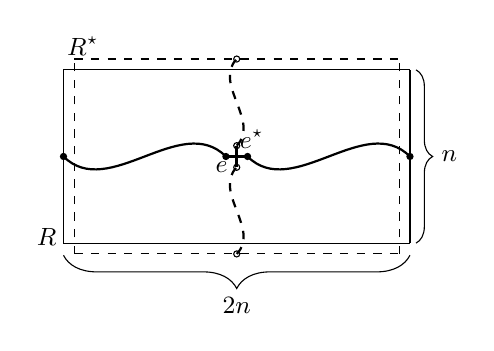
\begin{tikzpicture}[scale = 0.55]

	\draw[solid, black] (0, 0) -- (8, 0);
	\draw[solid, black] (0, 4) -- (8, 4);
	\draw[solid, black] (0, 0) -- (0, 4);
	\draw[solid, black] (8, 0) -- (8, 4);
	
	\draw[solid, very thick, black] (3.75, 2) -- (4.25, 2);
	\node[black] at (3.65, 1.75) {{\small $e$}};
	\draw[solid, very thick, black] (4, 1.75) -- (4, 2.25);
	\node[black] at (4.35, 2.40) {{\small $e^{\star}$}};
	
	
	\draw[dashed, black] (0.25, -0.25) -- (7.75, -0.25);
	\draw[dashed, black] (0.25, 4.25) -- (7.75, 4.25);
	\draw[dashed, black] (0.25, -0.25) -- (0.25, 4.25);
	\draw[dashed, black] (7.75, -0.25) -- (7.75, 4.25);
	
	\draw[solid, thick, black] (0, 2) to[out = -45, in = 135] (3.75, 2);
	\draw[solid, thick, black] (4.25, 2) to[out = -45, in = 135] (8, 2);
	\draw[fill] (3.75, 2) circle (2pt);
	\draw[fill] (4.25, 2) circle (2pt);
	\draw[fill] (0, 2) circle (2pt);
	\draw[fill] (8, 2) circle (2pt);
	
	\draw[dashed, thick, black] (4, -0.25) to[out = 45, in = -135] (4, 1.75);
	\draw[dashed, thick, black] (4,  2.25) to[out = 45, in = -135] (4, 4.25);
	\draw[draw] (4, 1.75) circle (2pt);
	\draw[draw] (4, 2.25) circle (2pt);
	\draw[draw] (4, -0.25) circle (2pt);
	\draw[draw] (4,  4.25) circle (2pt);
	
	\draw [decorate, decoration = {brace, amplitude = 12pt, mirror}, xshift = 0pt, yshift = -8pt] (0, 0) -- (8, 0) node [black, midway, xshift = 0pt, yshift = -18pt] {\small $2n$};
	
	\draw [decorate, decoration = {brace, amplitude = 6pt, mirror}, xshift = 4pt, yshift = 0pt] (8, 0) -- (8, 4) node [black, midway, xshift = 12pt, yshift = 0pt] {\small $n$};
	
	\node[black] at (-0.25, 0.15) {{\small $\text{R}^{\phantom{\star}}$}};
	\node[black] at (0.45, 4.55) {{\small $\text{R}^{\star}$}};
	
\end{tikzpicture}